\subsection{Примеры численного моделирования стабилизации неустойчивых решений}

\subsubsection{Стабилизация неустойчивых решений}

\newtheorem{exmp_stbur}{Пример}

\begin{exmp_stbur}
\end{exmp_stbur}

Пусть $\theta_0 = \frac{sin(\pi x)}{G(x)}$ - начальное условие. 
Параметр $\sigma$ возмем равный 15. В предыдущем параграфе показано неустойчивое 
поведение системы без управления, а сама стабилизация с параметрами 
$\omega = [0, 0.2], \; r = 15, \; m = 2$ предоставлена ниже


\begin{figure}[H]
  \centering
  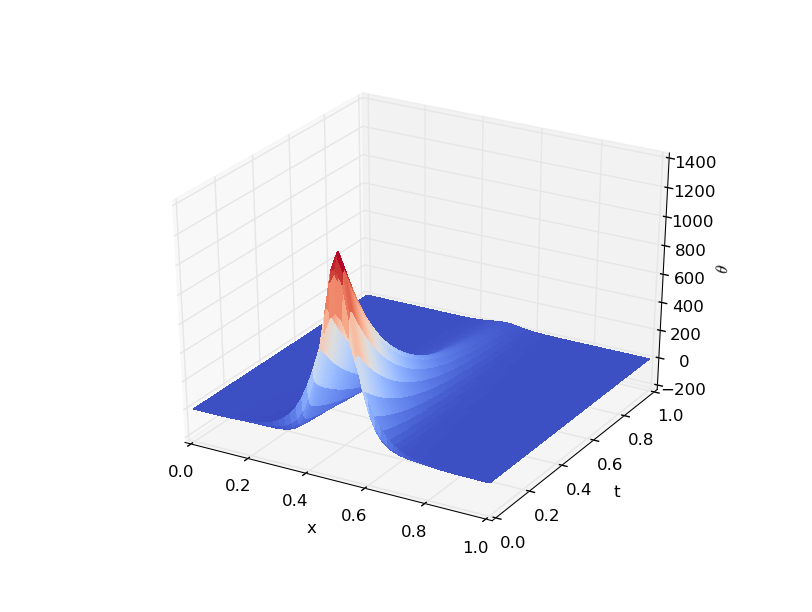
\includegraphics[width=4.5in]{re_s15}
  \caption{Управление с $m = 2, \; r = 15$}
  \label{fig:test2}
\end{figure}


%\begin{exmp_stbur}
%\end{exmp_stbur}
%В качестве начального условия возмем быстро осциллирующую функцию $\frac{\sin(10 \pi x)}{G(x)}$. Параметр $\sigma$ возмем равным 15. На рисунке 5 поведение системы без управления, рисунок 6 - управление с $\omega = [0, 0.2], \; r = 15, \; m = 2$.

%\begin{figure}[H]
%\centering
%\begin{minipage}{.5\textwidth}
  %\centering
  %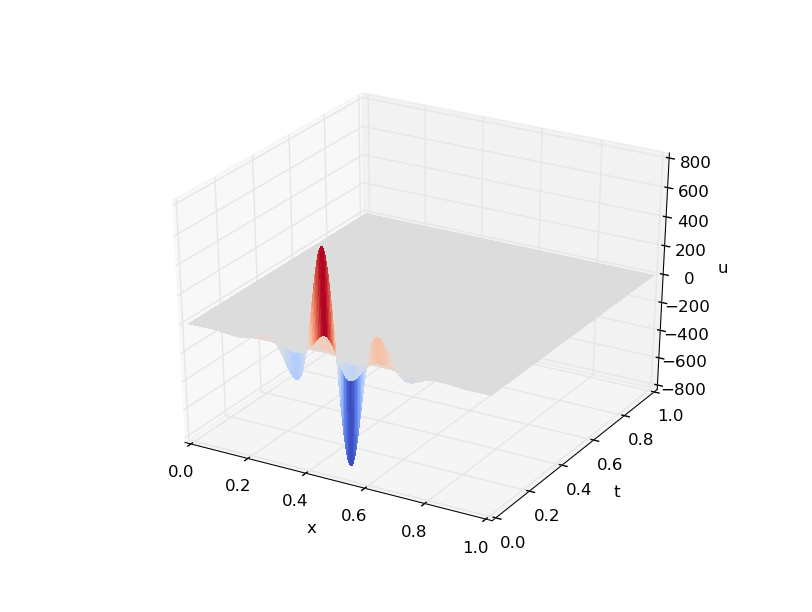
\includegraphics[width=3.5in]{ex_sin10_s15}
  %\caption{Без управления}
  %\label{fig:test1}
%\end{minipage}%
%\begin{minipage}{.5\textwidth}
  %\centering
  %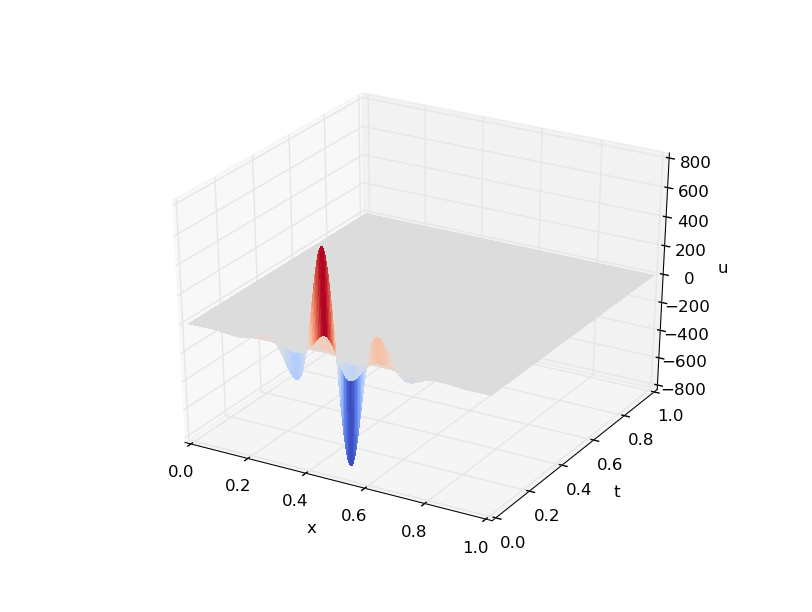
\includegraphics[width=3.5in]{re_sin10_s15}
  %\caption{Управление с $m = 2, \; r = 15$}
  %\label{fig:test2}
%\end{minipage}
%\end{figure}


\begin{exmp_stbur}
\end{exmp_stbur}
Пусть теперь начальное условие системы $\theta_0(x) = \frac{x^2}{G(x)}$.
Впспомним, что чем больше параметр $\sigma > 0$, тем сильнее он влияет на
неустойчивость нашей системы \eqref{fluct}. Зафиксируем следующие параметры
стабилизирующего оператора управления $\omega = [0, 0.2], \ r = 15$, а параметр 
$\sigma$  возмем равный $15$. Неустойчивость этой системы предемонстирована в
предыдущем параграфе (рис 2). Ниже представлен процесс стабилизации

\begin{figure}[H]
 \centering
  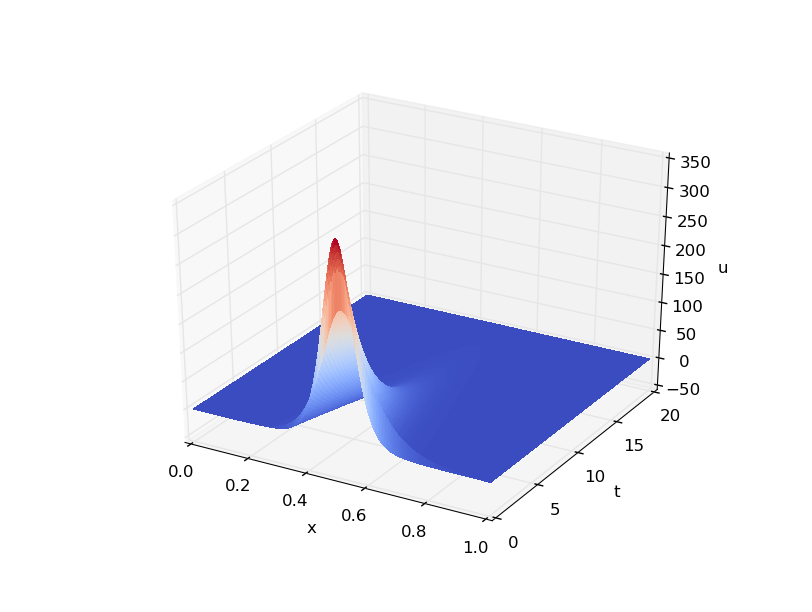
\includegraphics[width=4.5in]{re_x2_s15}
  \caption{$\omega = [0, 0.2], \; r = 15, \; m = 2$}
  \label{fig:test2}
\end{figure}

\subsubsection{Анализ параметров оператора стабилизации}

Рассмотрим ....

